% ----------------------------------------------------------
\chapter{Solução do modelo mecânico}
% ----------------------------------------------------------
A solução do modelo mecânico será feita através do \textit{software} ANSYS e a primeira parte desse capítulo descreverá a solução numérica pelo método dos elementos finitos (de forma mais genérica possível) comentando as opções do ANSYS, quando pertinente. Posteriormente, será dada ênfase na solução numérica envolvendo as do modelo constitutivo do material (que é o foco principal do trabalho). 

\section{Forma fraca das equações de campo}
No contexto da evolução quase estática e da hipótese das pequenas perturbações podem-se escrever as equações de campo na sua forma fraca através do princípio dos trabalhos virtuais. Sendo assim, aplicando um campo de deslocamento virtual $\dul$, cinematicamente admissível, em (\ref{eq:equilibrio_estatico_local}), porém ao longo de todo o volume $\Omega$ tem-se que:
\begin{equation}
	\label{eq:deslocamento_virtual}
	\int_{\Omega} \left(\divl \sigmall + \rho \fl \right)d\Omega \cdot \dul = 0,
\end{equation}
\begin{equation}
	\label{eq:deslocamento_virtual_2}
	\int_{\Omega} \divl \sigmall d\Omega \cdot \dul + \int_{\Omega} \rho \fl d\Omega \cdot \dul = 0.
\end{equation}

Aplicando o Teorema da Divergência no termo mais à esquerda da igualdade (\ref{eq:deslocamento_virtual_2}) obtém-se:
\begin{equation}
	\label{eq:deslocamento_virtual_3}
	\int_{\Omega} \sigmall : \dvarepsilonll d\Omega - \left(\int_{\Omega} \rho \fl \cdot \dul d\Omega + \int_{\partial \Omega} \Tl^d \cdot \dul dS \right) = U_{int} - W_{ext} = 0
\end{equation}

A expressão (\ref{eq:deslocamento_virtual}) é uma equação integral em que, no equilíbrio, o trabalho virtual das forças externas $W_{ext}$ sobre o sistema é totalmente convertido em energia potencial interna $U_{int}$  de deformação.

\section{Notação de Voigt}
Os tensores simétricos de segunda e quarta ordem são comumente representados, respectivamente, por arranjos (\textit{arrays}) vetoriais e matriciais convenientes à álgebra computacional. Dessa forma é utilizada a seguinte notação \cite[p. 682]{Zienkiewicz2005}:
\begin{equation}
	\label{eq:sigmal}
	\sigmall \rightarrow \sigmal = \left\{\sigma_{11}~~~\sigma_{22}~~~\sigma_{33}~~~\sigma_{21}~~~\sigma_{23}~~~\sigma_{31} \right\}^T
\end{equation}
\begin{equation}
	\label{eq:varepsilonl}
	\varepsilonll \rightarrow \varepsilonl = \left\{\varepsilon_{11}~~~\varepsilon_{22}~~~\varepsilon_{33}~~~2\varepsilon_{21}~~~2\varepsilon_{23}~~~2\varepsilon_{31} \right\}^T
\end{equation}
\begin{equation}
	\label{eq:Dl}
	\Dllll \rightarrow \Dll = 
	\begin{bmatrix}
		D_{1111} & D_{1122} & D_{1133}  & D_{1121} & D_{1123} & D_{1131} \\
				& D_{2222}  & D_{2233}  & D_{2221} & D_{2223} & D_{2231}  \\
				& 			& D_{3333}  & D_{3321} & D_{3323} & D_{3331}  \\
				& 			&		    & D_{2121} & D_{2123} & D_{2131}  \\
				& \text{SIM}&		    & 	       & D_{2323} & D_{2331}  \\
				& 			&		    & 	       &          & D_{3131} 
	\end{bmatrix}
\end{equation}
\begin{equation}
	\label{eq:dgdsl}
	\dgdsll \rightarrow \dgdsl = \left\{\dfrac{\partial g}{\partial \sigma_{11}}~~~\dfrac{\partial g}{\partial \sigma_{22}}~~~\dfrac{\partial g}{\partial \sigma_{33}}~~~\dfrac{\partial g}{\partial \sigma_{21}}~~~\dfrac{\partial g}{\partial \sigma_{23}}~~~\dfrac{\partial g}{\partial \sigma_{31}} \right\}^T
\end{equation}
\begin{equation}
	\label{eq:Uml}
	\Umll \rightarrow \Uml = \left\{1~~~1~~~1~~~0~~~0~~~0 \right\}^T
\end{equation}
\begin{equation}
	\label{eq:UmllotimesUll}
	\Umllll \rightarrow \Umll = 
	\begin{bmatrix}
		1 & 0 & 0 & 0 & 0 & 0 \\
		0 & 1 & 0 & 0 & 0 & 0  \\
		0 & 0 & 1 & 0 & 0 & 0  \\
		0 & 0 & 0 & 1/2 & 0 & 0  \\
		0 & 0 & 0 & 0 & 1/2 & 0  \\
		0 & 0 & 0 & 0 & 0 & 1/2 
	\end{bmatrix}
\end{equation}
\begin{equation}
	\label{eq:UmllotimesUll}
	\Umll \otimes \Umll \rightarrow  
	\begin{bmatrix}
		1 & 1 & 1 & 0 & 0 & 0 \\
		1 & 1 & 1 & 0 & 0 & 0  \\
		1 & 1 & 1 & 0 & 0 & 0  \\
		0 & 0 & 0 & 0 & 0 & 0  \\
		0 & 0 & 0 & 0 & 0 & 0  \\
		0 & 0 & 0 & 0 & 0 & 0 
	\end{bmatrix}
\end{equation}
sendo o subscrito $T$ a operação de transposição. Como se pode ver é utilizada a mesma simbologia de tensores de primeira ordem e de segunda ordem representando vetores (arranjos unidimensionais) e matrizes (arranjos bidimensionais), respectivamente. Nessa notação, as operações também são transformadas, de tal forma que:
\begin{equation}
	\label{eq:operacoes_voigt}
	\begin{array}{lcl}
		\underline{a} \cdot \underline{b} \rightarrow \underline{b}^T \underline{a}, \\ 
		\underline{\underline{a}} : \underline{\underline{b}} \rightarrow \underline{a}^T \underline{b}, \\ 
		\underline{\underline a} \otimes \underline{\underline b} \rightarrow \underline a ~ \underline b ^T, \\ 
		\underline{\underline{\underline{\underline{C}}}} : \underline{\underline{b}} \rightarrow \underline{\underline C} ~ \underline b, \\ 
		\underline{\underline{b}}:\underline{\underline{\underline{\underline{C}}}} : \underline{\underline{b}} \rightarrow \underline {b}^T \underline{\underline{C}} ~ \underline{b}, \\ 
		\left( 	\underline{\underline{\underline{\underline{C}}}}:\underline{\underline{a}} \right) \otimes \left( \underline{\underline{b}} :	\underline{\underline{\underline{\underline{C}}}} \right) \rightarrow \underline{\underline{C}}~ \underline{a}~\underline{b}^T \underline{\underline{C}}.
	\end{array}
\end{equation}

Além disso, na notação de Voigt, é necessário definir o produto termo-a-termo entre \textit{arrays} unidimensionais, de tal forma que:
\begin{equation}
	\label{eq:ab}
	\underline a ~ \underline b  = \underline c ~ \text{em que}~\underline c  = \left\{a_1b_1~~~a_2b_2~~~a_3b_3~~~a_4b_4~~~...~~~a_nb_n \right\}.
\end{equation}

Essa será a notação adotada para o restante do trabalho. Logo, o teorema dos trabalhos virtuais (\ref{eq:deslocamento_virtual_3}) pode ser reescrito da seguinte forma:
\begin{equation}
	\label{eq:deslocamento_virtual_3}
	\int_{\Omega} \dvarepsilonl^T \sigmal d\Omega - \left(\int_{\Omega} \rho \dul^T \fl d\Omega + \int_{\partial \Omega} \dul^T \Tl^d dS \right) = U_{int} - W_{ext} = 0
\end{equation}
\section{Discretização espacial em elementos finitos}
A solução por elementos finitos consiste em discretizar o domínio $\Omega$ em um conjunto de elementos contíguos $\Omega_e$, estabelecendo o que se chama de malha de elementos finitos (\autoref{discretizacao_MEF}). Cada elemento da malha tem um formato simples: linha, triângulo ou quadrilátero, tetraedro ou hexaedro, dependendo da dimensão (1D, 2D ou 3D) do domínio a ser discretizado. Cada elemento está conectado a outros elementos compartilhando "nós" sendo que a principal incógnita do problema são os deslocamentos nodais.
\begin{figure}[H]
	\begin{center}
		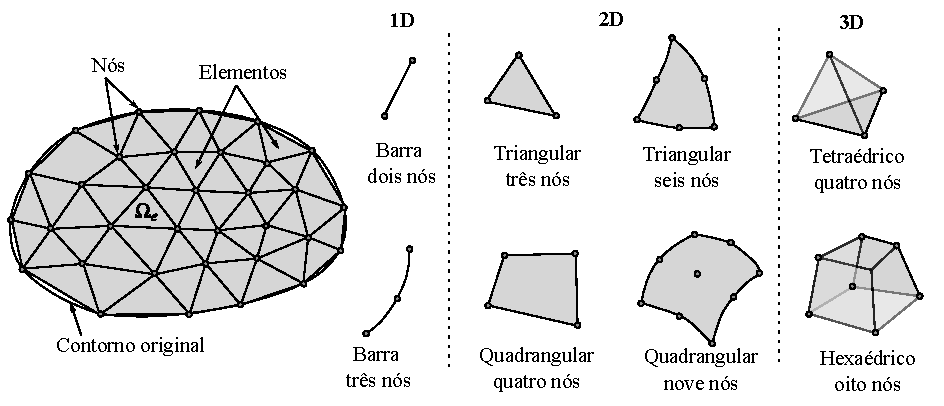
\includegraphics[scale = 1.0]{0601-discretizacao_dominio.pdf}
	\end{center}
	\caption{\label{discretizacao_MEF}Discretização de um domínio genérico em elementos finitos (adaptado de: \citeonline[p. 1-2]{DeSouza2003})}
\end{figure}

Nesse método, o campo de deslocamentos no interior dos elementos é relacionado com os deslocamentos nodais através de funções de interpolação, por exemplo, lineares ou quadráticas, cujos coeficientes são postos em função dos deslocamentos nodais. Dessa forma, o campo de deslocamentos no interior do elemento pode ser descrito como:
\begin{equation}
	\label{eq:campo_deslocamentos}
	\ul(\xl) = \ul(x_1,x_2,x_3) = \Nll(\xl)\ul_e.
\end{equation}
sendo $\ul(\xl)$ o campo de deslocamentos no interior do elemento, $\ul_e$ os deslocamentos nodais e $\Nll$ a matriz contendo as funções de interpolação (também conhecidas como funções de forma). A matriz $\Nll$  tem a seguinte estrutura:
\begin{equation}
	\label{eq:matriz_N}
	\Nll = 	\begin{bmatrix}
		N_1 & 0 & 0 & N_2 & 0 & 0 &  	& N_{n_e} & 0 & 0 \\
		0 & N_1 & 0 & 0 & N_2 & 0 & ... & 0 & N_{n_e} & 0  \\
		0 & 0 & N_1 & 0 & 0 & N_2 &  	& 0 & 0 & N_{n_e} 
	\end{bmatrix}_{n_d \times (n_e \cdot n_d)}
\end{equation}
em que $N_i$ são as funções de interpolação de cada nó $i$, $n_e$ número de nós do elemento e $n_d$ o número de dimensões. Introduzindo (\ref{eq:campo_deslocamentos}) nas equações de compatibilidade (\ref{eq:green_lagrange_linearizado}) tem-se:
\begin{equation}
	\label{eq:deformacoes}
	\varepsilonl(\xl) = \varepsilonl(x_1,x_2,x_3) = \nabla^s\ul(\xl) = \nabla^s \Nll~\ul_e = \Bll~\ul_e
\end{equation}
sendo $\varepsilonl$ o campo de deformações e $\Bll = \nabla^s \Nll$ a matriz que relaciona os deslocamentos nodais com as deformações no interior do elemento. Para problemas tridimensionais, o operador gradiente simétrico $\nabla^s$, na notação de Voigt, é dado por:
\begin{equation}
	\label{eq:gradiente_simetrico}
	\nabla^s = 	\begin{bmatrix}
		\dfrac{\partial}{\partial x_1} & 0 & 0  \\
		0 & \dfrac{\partial}{\partial x_2} & 0  \\
		0 & 0 & \dfrac{\partial}{\partial x_3} \\
		\dfrac{\partial}{\partial x_2} & \dfrac{\partial}{\partial x_1} & 0 \\
		0 & \dfrac{\partial}{\partial x_3} & \dfrac{\partial}{\partial x_2} \\
		\dfrac{\partial}{\partial x_3} & 0 & \dfrac{\partial}{\partial x_1}		
	\end{bmatrix}_{n_c \times n_d}
\end{equation}
em que $n_c$  é o número de componentes de deformações. Introduzindo (\ref{eq:deformacoes}) na lei de comportamento do material, é possível determinar as tensões no interior do elemento também em função dos deslocamentos nodais:
\begin{equation}
	\label{eq:tensoes}
	\sigmal(\xl) = \sigmal(x_1,x_2,x_3) = \Dll ~ \Bll ~\ul_e + \Dll ~\varepsilonl_0 + \sigmal_0
\end{equation}
na qual $\varepsilonl_0$ e $\sigmal_0$ são deformações e tensões iniciais no interior do elemento, respectivamente. Nos problemas de túneis, é através de $\sigmal_0$ que é introduzido as tensões \textit{in situ}. Para o caso de tensão geostática hidrostática, em um túnel de profundidade $H$ em um maciço com peso específico $\gamma_m$ a seguinte expressão é utilizada:
\begin{equation}
	\label{eq:tensoes_iniciais}
	\sigmal_0 = \gamma_m H \Uml
\end{equation}

Introduzindo as expressões (\ref{eq:campo_deslocamentos}), (\ref{eq:deformacoes}) e (\ref{eq:tensoes}) no princípio dos trabalhos virtuais (\ref{eq:deslocamento_virtual_3}), considerando o domínio de um elemento $\Omega_e$, obtém-se a seguinte equação de equilíbrio em forças:
\begin{equation}
	\label{eq:forcas_interna_externa}
	\Fl_{int_e} - \Fl_{ext_e} = \underline 0
\end{equation}
em que:
\begin{equation}
	\label{eq:forca_interna}
	\Fl_{int_e} = \int_{\Omega_e} \Bll^T \sigmal d\Omega_e = \Kll_e \ul_e + \Fl_{\varepsilon_{0_e}} + \Fl_{\sigma_{0_e}}
\end{equation}
\begin{equation}
	\label{eq:forca_externa}
	\Fl_{ext_e} = \Fl_{V_e} + \Fl_{S_e} + \Fl_{C_e} + \Fl_{N_e}
\end{equation}
nos quais:
\begin{equation}
	\label{eq:elementos_forca_interna}
	\Kll_e = \int_{\Omega_e} \Bll^T \sigmal d\Omega_e,~~~ \Fl_{\varepsilon_{0_e}} = \int_{\Omega_e} \Bll^T \Dll~ \varepsilonl_0 d\Omega_e,~~~ \Fl_{\sigma_{0_e}} = \int_{\Omega_e} \Bll^T \sigma_0 d\Omega_e,
\end{equation}
\begin{equation}
	\label{eq:elementos_forca_externa}
	\Fl_{V_e} = \int_{\Omega_e} \rho \Nll^T \fl d\Omega_e,~~~ \Fl_{S_e} = \int_{\partial \Omega_e} \Nll^T \Tl^d dS_e,~~~
	\Fl_{C_e} = \int_{\partial \Omega_{e}} \Nll^T \Tl^c dS_c,
\end{equation}
sendo que $\Fl_{int_e}$ e $\Fl_{ext_e}$ são as forças internas e externas no elemento, respectivamente, $\Kll_e$ a matriz de rigidez do elemento, $\Fl_{\varepsilon_{0_e}}$ e $\Fl_{\sigma_{0_e}}$  forças internas no elemento devido às deformações inciais e tensões iniciais, respectivamente, $\Fl_{V_e}$ forças de volume do elemento, $\Fl_{S_e}$ forças de superfície no contorno livre do elemento, $\Fl_{C_e}$ forças de contato entre elementos vizinhos e $F_{N_e}$  forças nodais. A Figura 6.2 ilustra as forças externas de um elemento genérico.
\begin{figure}[H]
	\begin{center}
		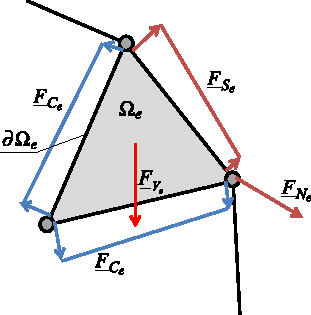
\includegraphics[scale = 1.0]{0602-diagrama de corpo livro de um elemento finito.pdf}
	\end{center}
	\caption{\label{discretizacao_MEF}Diagrama de corpo livre de um elemento finito (adaptado de: \citeonline[p. 19]{Lizarza2011})}
\end{figure}
No método dos elementos finitos, as integrais de volume no domínio  $\Omega_e$, por eficiência, são geralmente resolvidas em um domínio de referência $\Omega_\xi$ com geometria normalizada $-1 \le \xi_i \le 1$. As coordenadas $\underline \xi$ também são conhecidas como coordenadas naturais do elemento. Portanto, é feita a seguinte troca de variáveis nas integrais de volume \cite[p. 147]{Zienkiewicz2005}:
\begin{equation}
	\label{eq:troca_variavel_integral_volume}
	\int_{\Omega_e}d\Omega_e = \iiint dx_1 dx_2 dx_3 = \int_{\Omega_\xi}det(\Jll)d\Omega_\xi = \int_{-1}^{1}\int_{-1}^{1}\int_{-1}^{1}\text{det}(\Jll)d\xi_1d\xi_2d\xi_3
\end{equation}
em que $\Jll = \dfrac{\partial \xl}{\partial \xil}$  é o Jacobiano da transformação entre as coordenada $\xl$ e $\xil$, sendo calculado com as mesmas funções de interpolação usadas para os deslocamentos no interior do elemento, se tratando, portanto, de um \textbf{elemento isoparamétrico}. A integral assim representada é então resolvida pelo método da Quadratura de Gauss-Legendre. Portanto, para uma função $f(\xl)$ qualquer, no domínio $\Omega_e$, tem-se:
\begin{equation}
	\label{eq:troca_variavel_integral_volume}
	\int_{\Omega_e}f(\xl)d\Omega_e = \int_{-1}^{1}\int_{-1}^{1}\int_{-1}^{1}f(\xil)\text{det}(\Jll)d\xi_1d\xi_2d\xi_3 = \sum_{i_p=1}^{n_p}W_{i_p}J_{i_p}f(\xil_{i_p})
\end{equation}
em que $n_p$ é o número de pontos de integração (ou pontos de Gauss), $W_{i_p}$ é o peso referente ao ponto de integração, $f(\xil_{i_p})$ é o valor da função nas coordenadas naturais do ponto de integração e $J_{i_p}$ é o determinante do Jacobiano da transformação (nas coordenadas do ponto de integração) dado por \cite[p. 206-207]{Zienkiewicz2005}:
\begin{equation}
	\label{eq:jacobiano_transformacao}
	J_{i_p} = \left\{
	\begin{array}{lcl}
		 \text{det}(\Jll)_{i_p}~~~\text{em 3D e estado plano de deformações} \\
		2\pi\xi_{r_{i_p}}\text{det}(\Jll)_{i_p} ~~~\text{em axissimetria}
	\end{array}
\right..
\end{equation}
sendo $\xi_{r_{i_p}}$ a coordenada radial natural do ponto de Gauss. A equação (6.26) integra  exatamente se este for um polinômio de ordem menor ou igual a $2n_p-1$.

Os elementos finitos que serão utilizados nesse trabalho com suas funções de interpolação, pesos e coordenadas dos pontos de integração podem ser vistos na \autoref{PLANE183}, para análises em estado plano de deformações e axissimetria e, para análises tridimensionais, que consomem maior tempo de processamento, será utilizado o elemento da \autoref{SOLID185}.
\begin{figure}[H]
	\begin{center}
		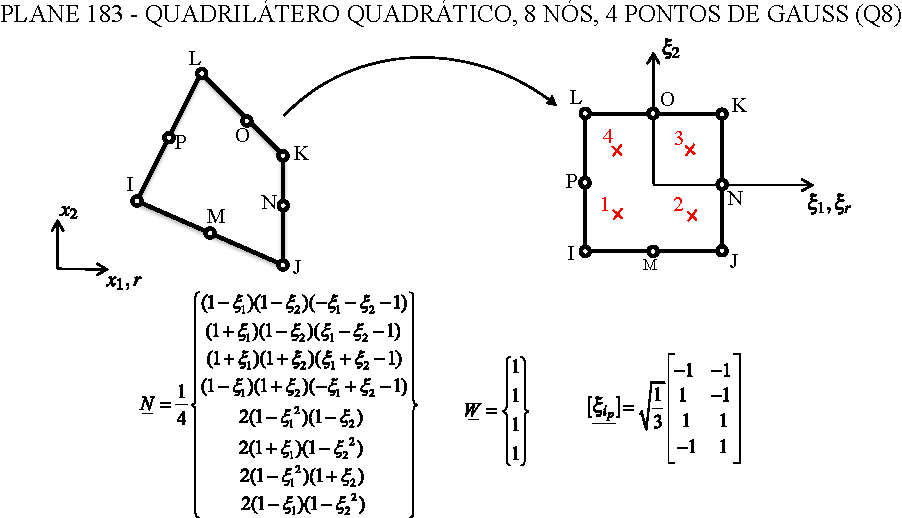
\includegraphics[scale = 1.0]{0603-quadrilatero quadratico.pdf}
	\end{center}
	\caption{\label{PLANE183}Funções de interpolação, pesos e coordenadas dos pontos de Gauss para o elemento quadrilátero quadrático \textit{serendipity} isoparamétrico (adaptado de: \citeonline[p. 337, 369-370]{ANSYS2018})}
\end{figure}
\begin{figure}[H]
	\begin{center}
		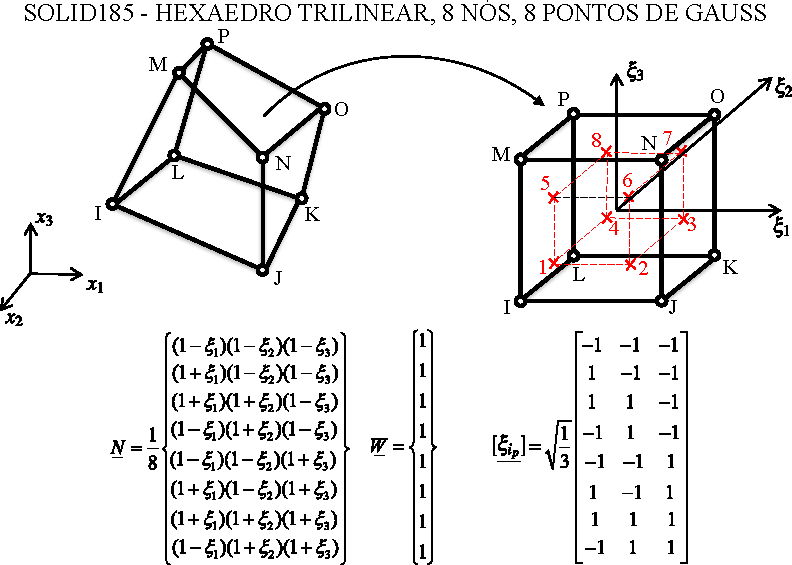
\includegraphics[scale = 1.0]{0604-hexaedro linear.pdf}
	\end{center}
	\caption{\label{SOLID185}Funções de interpolação, pesos e coordenadas dos pontos de Gauss para o elemento hexaedro trilinear isoparamétrico (adaptado de: \citeonline[p. 345, 369-370]{ANSYS2018})}
\end{figure}

No ANSYS, ambos elementos possuem a opção degenerada em que é possível trabalhar de forma colapsada, triangular, por exemplo, no caso do PLANE183, e prisma, tetraédrica ou piramidal, no caso do SOLID185. Nas análises não serão utilizadas essas formas. 

O elemento SOLID185 possuí também opções que lidam com problemas de travamento (\textit{Locking}) e modos espúrios (\textit{Hourglass}). O travamento é caracterizado por uma rigidez excessiva do elemento, e ocorre principalmente em elementos de primeira ordem com integração completa que estão sujeitos a flexão. Ou ainda, quando o material é quase incompressível. Também podem ocorrer em elementos de segunda ordem, quando as deformações plásticas são da ordem das deformações elásticas. Esse problema evita-se com refinamento da malha, técnicas de subintegração e funções de formas extras. O ANSYS possuí as duas últimas técnicas para o SOLID185 (\textit{Uniform Reduced Integration with Hourglass Control} e \textit{Enhanced Strain Formulation}). Os modos espúrios ocorrem quando se utiliza as técnicas de subintegração e é caracterizado por uma distorção no elemento porém com zero deformação. Esse problema é evitado utilizando integração completa ou refinamento da malha. No presente trabalho se utilizará a \textbf{integração completa} (\textit{Full integration with B method}) e se tentará evitar esses problemas através do \textbf{refinamento da malha}. 

\section{Solução do sistema não linear}

Após o processo de discretização do domínio $\Omega$ é necessário fazer a montagem e a solução do seguinte sistema global de equações:
\begin{equation}
	\label{eq:sistema_global}
	\left(\Kll~\ul + \Fl_{\varepsilon_{0}} + \Fl_{\sigma_{0}}\right) - \left(\Fl_V+\Fl_S+\Fl_N \right) = \Fl_{int} - \Fl_{ext} = f(\ul) = \underline{0}  
\end{equation}
em que $\Kll$ é a matriz de rigidez global resultante da montagem das matrizes de rigidezes $\Kll_e$ de cada elemento, $\ul$ é o vetor incógnito de deslocamentos nodais global proveniente da montagem dos deslocamentos nodais $\ul_e$ de cada elemento, $\left\{\Fl_V,\Fl_S,\Fl_N,\Fl_{\varepsilon_0},\Fl_{\sigma_0} \right\}$ são as forças globais resultantes da montagem das forças em cada elemento, conforme (\ref{eq:elementos_forca_interna}) e (\ref{eq:elementos_forca_externa}). Não haverá um vetor de forças de contato global $\Fl_C$, uma vez que as forças de contato entre elementos vizinhos possuem a mesma magnitude e sentidos contrários e, portanto, se anulam no somatório global.

Quando há uma não linearidade envolvendo as leis constitutivas do material (tal como na plasticidade ou viscoplasticidade, em que o problema é dependente da trajetória das tensões), a matriz de coeficientes $\Kll$ passa a depender dos deslocamentos nodais incógnitos  $\ul$, tornando o sistema (\ref{eq:sistema_global}) não linear. O \textbf{método de Newton-Raphson} (NR) é o processo iterativo comumente utilizado para resolver esse sistema e é utilizado pelo ANSYS. Dessa forma, aproximando (\ref{eq:sistema_global}) por uma série de Taylor truncada na primeira ordem (linearização) tem-se:
\begin{equation}
	\label{eq:taylor}
	\fl(\ul) \approx \fl(\ul_i) + \fl'(\ul_i)(\ul_{i+1}-\ul_i).
\end{equation}

Fazendo $\fl(\ul) = \underline{0}$, isolando $\ul_{i+1}$ e substituindo (\ref{eq:sistema_global}) em (\ref{eq:taylor}), considerando que $\Fl_{ext}$ não depende dos deslocamentos (devido à hipótese das pequenas perturbações), tem-se a seguinte expressão iterativa para aproximar $\ul$:
\begin{equation}
	\label{eq:NR}
	\ul_{i+1} = \ul_i - \Kll(\ul_i)^{-1}\left(\Fl_{int}(\ul_i)-\Fl_{ext} \right) = \ul_i - \Kll_i^{-1} \left(\Fl_{int_i} - \Fl_{ext} \right) = \ul_i + \Kll_i^{-1}\Rl_i = \ul_i + \Delta \ul_i
\end{equation}
em que $\Delta \ul_i$ é o incremento de deslocamentos nodais da iteração atual $i$, $\Fl_{int_i}$ são as forças internas (ou forças restauradoras) da iteração atual (calculadas com $\ul_i$), $\Rl_i$ é o vetor de carga desbalanceado (também chamado de resíduo) para a iteração atual, $\Kll_i$ a matriz de rigidez global tangente na iteração atual, $\ul_i$ os deslocamentos nodais na iteração atual e $\ul_{i+1}$ os deslocamentos nodais atualizados para a próxima iteração.

Como $\Delta \ul_i = \Kll_i^{-1}\Rl_i$ é um sistema de equações esparso (contém muitos elementos nulos) e geralmente simétrico, há diversas técnicas de solução que buscam explorar essas características para obter eficiência computacional. O ANSYS possui uma técnica de \textbf{solução direta}, que busca resolver o sistema através de operações que compreendem a inversão da matriz de rigidez, e três técnicas de \textbf{soluções indiretas}, que se aproximam da solução do sistema de forma interativa com uma dada tolerância.

A solução direta (\textit{SPARSE - Sparse Direct Solver}) consiste em aplicar a fatorização de Cholesky modificada $\Kll = \Lll~\Dll~ \Lll^T$ (em que $\Lll$ é uma matriz triangular inferior e $\Dll$ uma matriz diagonal) e, através de substituições progressivas e retroativas, resolver o sistema. Algoritmos de solução direta podem ser encontrados em \citeonline{Felippa1975} e \citeonline{Smith2014}.

As soluções indiretas, implementadas no ANSYS, se baseiam na família de Métodos dos Gradientes Conjugados Pré-Condicionados, que consistem em minimizar o potencial $V(\Delta \ul) = \frac{1}{2}\Delta \ul^T\Kll~\Delta \ul - \Delta \ul^T\Rl$ com aproximações $\Delta \ul^{(j+1)}=\Delta \ul^{j} + a_j \underline{d}^{(j)}~\text{para}~j=0,1,2,..m$, sendo $\underline d^{(j)}$ os gradientes conjugados, ou seja, $\underline {d}^{{(i)}^T} \Kll d^{(j)} = 0,~~ \forall i \neq j$. Quando o sistema é bem condicionado, sua solução converge para $m \leq n_{gdl}$ iterações e o número de operações é proporcional à raiz quadrada do número de condição da matriz $\Kll$, numero este que é a razão entre o maior e menor autovalor da matriz $\Kll$. Em vista disso, há diversas técnicas de transformação do sistema para melhorar o condicionamento dessa matriz através de uma transformação do tipo $\Mll^{-1}\Kll~\ul = \Mll^{-1} \Rl$, em que $\Mll$ é o pré-condicionador. O ANSYS possuí três métodos \cite[p. 647]{ANSYS2018}:

\begin{alineas}
	
	\item JCG (\textit{Jacobi Conjugate Gradiente}): o pré-condicionador é tomado como sendo uma matriz diagonal cujos termos são as diagonais da matriz de rigidez;
	
	\item ICCG (\textit{Incomplete Cholesky Conjugate Gradiente}), o pré-condicionador é tomado através de uma fatorização incompleta de Cholesky. O algoritmo é internamente desenvolvido pela ANSYS e não publicado, e é mais robusto que o primeiro para matrizes mal condicionadas;
	
	\item PCG (\textit{Preconditioned Conjugate Gradiente}) é um solucionador da \textit{Computational Applications and System Integration, Inc} que não consta nos manuais do \textit{software}. Contudo, é dito eficiente e confiável para problemas mal condicionados.
	
\end{alineas}

Maiores explicações dessas soluções indiretas, podem ser encontrados em \citeonline[p. 316]{Mendonca2019}. Cabe salientar que, tanto os métodos diretos quanto indiretos, são implementados buscando a eficiência computacional, evitando-se trabalhar com os elementos nulos, diminuindo o armazenamento e o número de operações. Alguns métodos que compreendem reordenamento e armazenamento eficiente do sistema, utilizados pelo ANSYS, podem ser encontrados em \citeonline{George1981}. Além disso, uma vantagem do ANSYS é a possibilidade de trabalhar com computação de alto desempenho (\textit{High Performance Computing}) com opções de aceleração usando placas de vídeo da Nvidia, memória compartilhada (SMP - \textit{Shared-Memory Parallel}) ou computação distribuída (MPI - \textit{Message Passing Interface}). Para o presente trabalho, foi utilizado a opção de SMP com 12 processadores.

A rigor para um problema não linear a escolha do melhor método de solução vai depender de testagem. Por padrão o ANSYS utiliza o SPARSE. Contudo, recomenda utilizar o método PCG para estruturas sólidas 3D que possuem mais de 200.000 graus de liberdade. Para problemas mal condicionados, seja pela forma dos elementos, grandes diferenças entre as propriedades dos materiais ou ainda por insuficiente condições de contorno, recomenda-se o SPARSE \cite[p. 242]{ANSYS2018b}.

Para incorporar a dependência do histórico de cargas/tempo, para um dado passo de carga/tempo $p$, a expressão (\ref{eq:NR}) é discretizada em $1 \leq n \leq n_s$ subpassos em que a carga externa e o tempo do passo são incrementados linearmente. Dessa forma, itera-se o sistema (\ref{eq:NR}) repetidas vezes para cada subpasso $n$ tendo-se:
\begin{equation}
	\label{eq:NR1}
	\Delta \ul_{n,i} = \Kll_{n,i}^{-1}\left(\Fl_{ext_{n+1}} - \Fl_{int_{n,i}} \right) = \Kll_{n,i}^{-1}\Rl_{n,i},
\end{equation}
\begin{equation}
	\label{eq:NR2}
	\ul_{n,i+1} = \ul_{n,i}+\Delta\ul_{n,i},
\end{equation}
\begin{equation}
	\label{eq:NR3}
	\Fl_{ext_{n+1}} = \Fl_{ext_n} + \Delta \Fl_{{ext}_p},
\end{equation}
\begin{equation}
	\label{eq:NR4}
	t_{n+1} = t_n + \Delta t_p,
\end{equation}
em que
\begin{equation}
	\label{eq:NR5}
	\Fl_{int_{n,i}} = \left( \int_{\Omega} \Bll^T \sigmal d\Omega \right)_{n,i}
\end{equation}
sendo $\ul_{0,0}$, $\Fl_{int_{0,0}}$, $\Fl_{ext_0}$   e $t_0$ nulos. Para os próximos subpassos os valores de $\ul_{n,0}$ e $\Fl_{int_{n,0}}$, correspondem aos valores da solução convergente no subpasso anterior $n-1$. O número de subpassos $n_s$ e o incremento de força externa $\Delta \underline{F}_p$ são dependentes do incremento de tempo utilizado no passo $\Delta t_p$, e são dados por:
\begin{equation}
	\label{eq:NR6}
	n_s = \dfrac{t_p}{\Delta t_p},~~~ \Delta \Fl_{p} = \dfrac{\Fl_{ext_p}}{n_s}
\end{equation}
sendo $t_p$ e $\Fl_{ext_p}$, nessa ordem, o tempo e a força no final do passo. Em busca da convergência e eficiência computacional, o ANSYS tem a opção de variar automaticamente o $\Delta t_p$ dentro de um intervalo $\Delta t_{p_{min}} \leq \Delta t_p \leq \Delta t_{p_{max}}$ fornecido pelo usuário. É possível que o algoritmo não convirja durante as iterações e, portanto, é utilizado um limite de $n_{eqit} = 25$ iterações de equilíbrio por subpasso. Quando a solução não converge dentro desse limite, o ANSYS divide pela metade o incremento de tempo, e consequentemente a carga, e reinicia o cálculo do passo. Esse procedimento é chamado de Método da Bisseção e é executado tantas vezes quanto necessárias até atingir a convergência ou $\Delta t_p \leq \Delta t_{p_{min}}$ a partir do qual a solução é dada como não convergente e estabelecido o critério de parada \cite[p. 637]{ANSYS2018}.

A convergência é verificada sobre o vetor resíduo e o incremento de deslocamentos nodais para cada iteração de equilíbrio, através das seguintes expressões (omitindo-se o subíndice $n$) \cite[p. 667]{ANSYS2018}:
\begin{equation}
	\label{eq:convergencia}
	||\Rl_i|| \leq \varepsilon_R R_{ref},~~~ ||\Delta \ul_i || \leq \varepsilon_u u_{ref}
\end{equation}
em que $\varepsilon_R$ e $\varepsilon_u$ são as tolerâncias para o resíduo (de 0,5\%) e deslocamentos (de 5\%), respectivamente. Os valores de referência $R_{ref}$ e $u_{ref}$ são $||\Fl_{ext_p}||$ e $||\ul_{n,i}||$, respectivamente. Ou seja, por padrão o critério para o resíduo é de 0,5\% do valor das forças externas e os deslocamentos não podem apresentar uma variação maior do que 5\%. No ANSYS, a norma pode ser calculada de três formas: a máxima componente em valor absoluto, a soma absoluta das componentes ou a norma euclidiana das componentes, conforme:
\begin{equation}
	\label{eq:jacobiano_transformacao}
	||\xl|| = \left\{
	\begin{array}{lcl}
		||\xl||_\infty = \text{max}(x_j) \\
		||\xl||_1 = \sum_{j}|x_j| \\
		||\xl||_2 = (\sum_{j}x_j^2)^{1/2}
	\end{array}
	\right..
\end{equation}
em que $j$ é o índice da componente do vetor $\xl = \Rl$ e $\xl = \Delta \ul$. Para o presente trabalho foi escolhida a norma euclidiana que era o padrão do ANSYS. A \autoref{NR} ilustra o andamento da solução ao longo dos subpassos. Pode-se ver que o resíduo e o incremento de deformações vão ficando cada vez menores ao longo das iterações de equilíbrio.
\begin{figure}[H]
	\begin{center}
		\includegraphics[scale = 1.0]{0605-ilustracao das iteracoes do método de NR.pdf}
	\end{center}
	\caption{\label{NR}Ilustração das iterações do método de Newton-Raphson (adaptado de: \citeonline[p. 301]{Chen1988})}
\end{figure}

O ANSYS possui ainda três variações do método de Newton-Raphson de acordo com a estratégia de atualização da matriz de rigidez $\Kll_{n,i}$ (\citeyear{ANSYS2018}, p. 666): 
\begin{alineas}
	
	\item \textbf{Completo} (\textit{Full}): quando a matriz de rigidez é atualizada a cada iteração $i$, ou seja, $\Kll_{n,i} \leftarrow \Kll_{n,i}$. Essa opção reduz o número de iterações de equilíbrio (convergência quadrática), porém, exige a montagem, fatorização e inversão da matriz a cada iteração;
	
	\item \textbf{Modificado} (\textit{Modified}): quando a matriz de rigidez é atualizada apenas a cada subpasso de carga/tempo $n$, ou seja, $\Kll_{n,i} \leftarrow \Kll_{n,0}$; 
	
	\item \textbf{Inicial} (\textit{Inicial Stiffness}): quando é utilizada a mesma matriz para todos os subpassos e iterações, ou seja, $\Kll_{n,i} \leftarrow \Kll_{0,0}$. 
	
\end{alineas}

Além dessas opções, para problemas estáticos, o ANSYS possui três técnicas para melhorar a convergência do método de Newton-Raphson, que são \cite[p. 668-673]{ANSYS2018}:

\begin{alineas}
	\item \textbf{Preditor} (\textit{Predictor}): extrapola o vetor de deslocamentos iniciais de cada subpasso utilizando os incrementos de deslocamentos acumulados do subpasso anterior multiplicados pela relação entre os incrementos de tempo entre ambos subpassos;
	
	\item \textbf{Descida Adaptativa} (\textit{Adaptative Descent}): consiste em alternar entre a matriz de rigidez tangente e secante conforme o andamento do resíduo durante as iterações de equilíbrio. Só é utilizada em conjunto com o método de Newton-Raphson Completo;
	
	\item \textbf{Pesquisa de linha} (\textit{Line Search}): tenta melhorar a solução multiplicando o incremento de deslocamentos por um escalar determinado pela minimização da energia do sistema;
	
	\item \textbf{Método do comprimento de arco} (\textit{Arc-Length Method}): utilizado para solução de equilíbrio estático não-linear de problemas instáveis como flambagem e pós-flambagem.
	
\end{alineas}

Na \autoref{NR-fluxograma} tem-se o fluxograma do método de Newton-Raphson, mostrando as três opções de atualização da matriz de rigidez, o método da bisseção e os laços das iterações de equilíbrio e de subpassos.
\begin{figure}[H]
	\begin{center}
		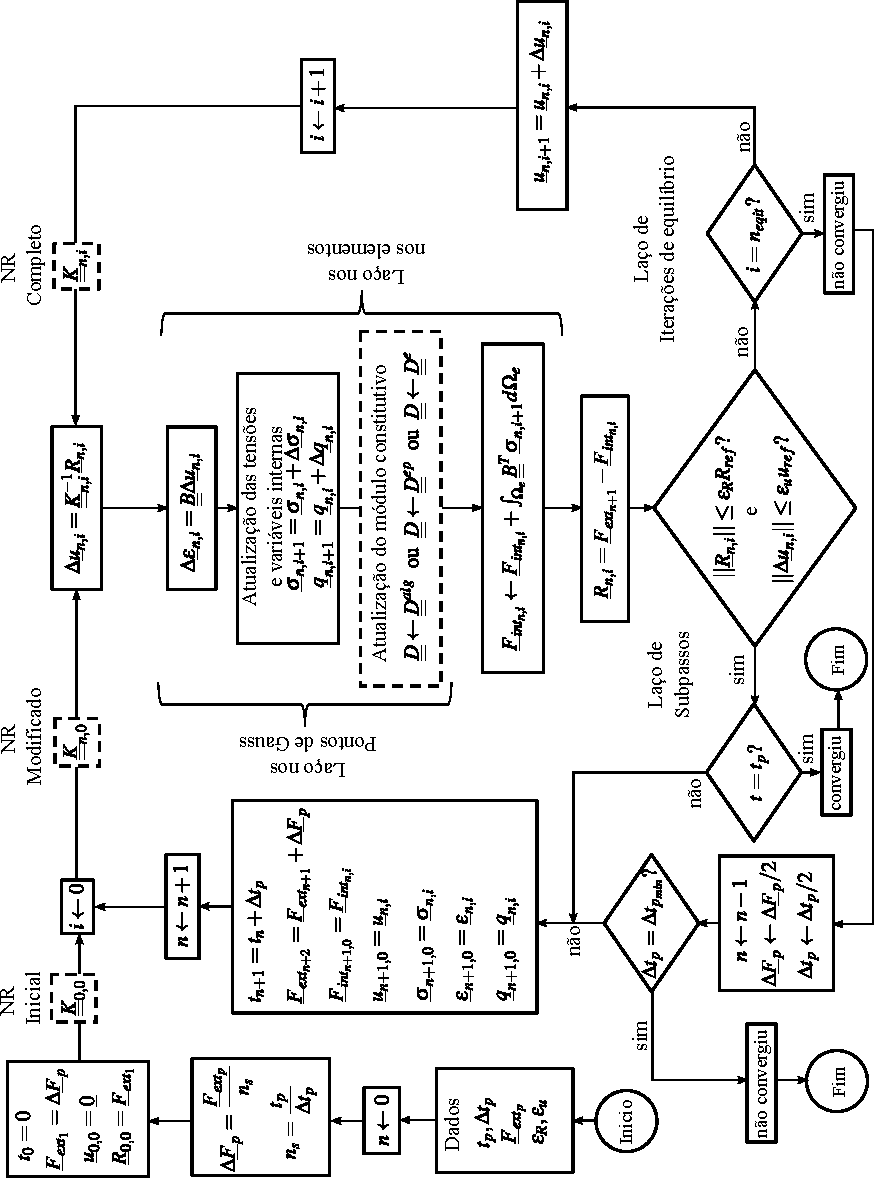
\includegraphics[scale = 1.0]{0606-fluxograma do metodo NR.pdf}
	\end{center}
	\caption{\label{NR-fluxograma}Fluxograma do método de Newton-Raphson para solução do sistema de equações globais não lineares}
\end{figure}
Ainda na \autoref{NR-fluxograma} está detalhado a parte de atualização das tensões e variáveis internas e do módulo constitutivo, que serão os temas do próximo capítulo. É importante que esteja nesse fluxograma o detalhe dos laços nos elementos e nos pontos de Gauss, pois a customização do modelo do material, através da subrotina USERMAT, como veremos, estará justamente aninhado nesse laço mais interno dos pontos de Gauss.

A convergência quadrática da opção de Newton-Raphson Completo só é efetivamente obtida se for utilizado o módulo consistente $\Dll^{alg}$ após o algoritmo de integração das tensões, conforme \citeonline{Simo1985}.


\section{Algoritmo de atualização das tensões e variáveis internas}

\subsection{Integração das equações constitutivas elastoplásticas}


\subsubsection{Esquema de integração totalmente implícito}


\subsubsection{Esquema de integração semi-implícito}


\subsection{Atualização do módulo constitutivo}

\subsection{Particularizando para estado plano de deformações e axissimetria}

\subsection{Domínios, discretização, condições de contorno e ciclo construtivo para os modelos de verificação}


